\begin{frame}
\frametitle{Correlation is not causation - the importance of understanding what drives model prediction}
\begin{columns}
    \begin{column}{0.67\textwidth}
        \begin{itemize}
            \item In the mid 1990s a group of researchers led by Tom Mitchel produced state-of-the-art neural network models for predicting risk of death from pneumonia. This was to be used to select patients for more intensive care.
            \item They were surprised to see that a history of asthma was associated with lower risk of death.
            \item After discussion with clinicians they concluded that asthma patients have lower mortality because they will receive more intensive care, not because pneumonia is less serious.
        \end{itemize}
    \end{column}
    \begin{column}{0.3\textwidth}
        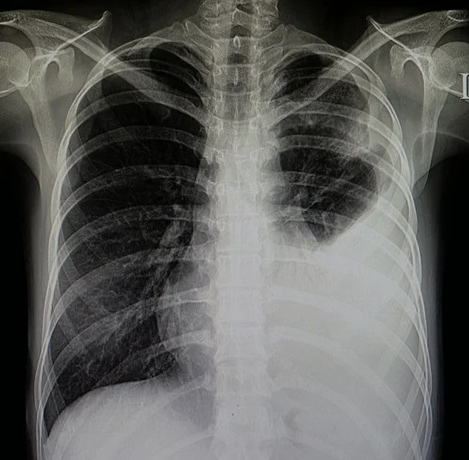
\includegraphics[width=1\textwidth]{./misc_images/pneumonia.png}
    \end{column}
\end{columns}
\end{frame}